\documentclass[11pt,a4paper]{article}

% ---------- Packages ----------
\usepackage[margin=2.2cm]{geometry}
\usepackage[T1]{fontenc}
\usepackage{lmodern}
\usepackage{amsmath,amssymb}
\usepackage{graphicx}
\usepackage{booktabs}
\usepackage{subcaption}
\usepackage{float}
\usepackage{xcolor}
\usepackage[colorlinks=true,linkcolor=blue!60!black,urlcolor=blue!60!black,citecolor=blue!60!black]{hyperref}
\usepackage{enumitem}
\setlist{nosep,leftmargin=*}

% Figures live in ../results (generated by train.py); on Overleaf put them in results/ or the root
\graphicspath{{../results/}{results/}{./}}

\newcommand{\repo}{\url{https://github.com/DINESH3803/ML_Assignment}}

\title{\textbf{Assignment-1: Polynomial Regression}}
\author{Dinesh Karthik (BT2024199)\\[4pt]
\small GitHub repository: \repo}
\date{}

\begin{document}
\maketitle
\vspace{-1.5em}

% =====================================================================
\section{Introduction}
The task is to predict a continuous target $y$ for two personalised datasets using
\emph{only} polynomial regression:
\begin{itemize}
  \item \textbf{var1 -- Steam turbine optimisation:} six operational parameters
        $x_1,\dots,x_6$ $\rightarrow$ Net Power Score (moderate degree, $\le 10$).
  \item \textbf{var2 -- Thermal reservoir mapping:} three spatial offsets
        $x_1,x_2,x_3$ $\rightarrow$ Thermal Anomaly Score (high degree, $\le 20$).
\end{itemize}
A polynomial of degree $d$ contains every monomial
$x_1^{p_1}\cdots x_n^{p_n}$ with $\sum_i p_i \le d$, so for $n$ features it has
$\binom{n+d}{d}-1$ non-constant terms. The number of terms grows quickly with $d$
(e.g.\ 461 terms for $n{=}6, d{=}5$), so the main challenge is choosing a degree
that avoids both underfitting and overfitting. Models are evaluated on hidden test
labels using MSE and $R^2$.

% =====================================================================
\section{Data Exploration}
Each problem has 1000 training rows and 1000 test rows. All inputs lie in
$[-1,1]$, and a large fraction of values sit \emph{exactly} at $\pm1$, which
suggests the data were clipped.

\begin{table}[H]
\centering
\small
\begin{tabular}{lcccc}
\toprule
 & Features & $y$ mean $\pm$ std & Fraction at $\pm1$ (train) & Fraction at $\pm1$ (test) \\
\midrule
var1 & 6 & $0.97 \pm 3.21$ & 0.30--0.34 & 0.48--0.51 \\
var2 & 3 & $2.61 \pm 6.94$ & 0.25--0.26 & 0.23--0.26 \\
\bottomrule
\end{tabular}
\caption{Dataset summary.}
\label{tab:data}
\end{table}

Key observations:
\begin{itemize}
  \item \textbf{Weak linear signal.} Pearson correlations with $y$ are small
        (var1: $|r|\le0.27$; var2: $|r|\le0.47$). A degree-1 model explains only
        about 10\% (var1) and 23\% (var2) of the variance, so the relationship is
        strongly non-linear and depends on interactions between features.
  \item \textbf{Covariate shift in var1.} The var1 test set has many more clipped
        values than the training set (about 50\% vs.\ 32\% per feature). The typical
        row has 2 clipped features in train but 3--4 in test. The test set therefore
        sits closer to the edges of the hypercube, where high-degree polynomials
        tend to extrapolate badly. var2 shows no such shift.
\end{itemize}

% =====================================================================
\section{Methodology}

\subsection{Model}
Every model is the following scikit-learn pipeline:
\[
\texttt{PolynomialFeatures}(d) \;\rightarrow\; \texttt{StandardScaler} \;\rightarrow\; \texttt{Ridge}(\alpha).
\]
\begin{itemize}
  \item \textbf{Polynomial expansion} creates all monomials up to total degree $d$,
        including cross terms. The model is still linear in its parameters, so it
        remains a polynomial regression.
  \item \textbf{Standardisation.} Higher powers have very different scales, so each
        expanded feature is scaled to zero mean and unit variance. This makes the
        problem better conditioned and lets a single $\alpha$ penalise all terms
        fairly.
  \item \textbf{Ridge ($L_2$) regularisation} minimises
        $\|y - X\beta\|_2^2 + \alpha\|\beta\|_2^2$. Ridge does not change the model
        family; it only shrinks the coefficients. This keeps high-degree fits stable
        even when the number of terms approaches the number of training rows, which
        is where plain least squares breaks down. $\alpha \to 0$ recovers OLS.
\end{itemize}

\subsection{Model selection}
\begin{itemize}
  \item \textbf{Grid search} over $(d,\alpha)$:
        var1: $d\in\{2,\dots,8\}$, $\alpha\in[10^{-3},10^{3}]$ (13 log-spaced values);
        var2: $d\in\{4,\dots,18\}$, $\alpha\in[10^{-4},10^{2}]$ (13 values).
  \item \textbf{Repeated 5-fold cross-validation} (3 repeats, seed 42, i.e.\ 15
        train/validation splits per configuration). Repeating the folds reduces the
        variance of the error estimate and gives a standard deviation for each score.
  \item \textbf{Selection criterion:} the configuration with the lowest mean
        validation MSE. The chosen pipeline is then refit on the full training set
        and used to predict the test set.
\end{itemize}

% =====================================================================
\section{Problem 1 (var1): Steam Turbine}

\subsection{Unregularised baseline}
An OLS degree sweep (Table~\ref{tab:v1ols}) shows the classic bias--variance
trade-off. Training error falls steadily as the degree grows, but validation error
reaches its minimum at $d{=}4$ and then rises sharply at $d{=}5$, where the 461
terms leave only about 1.7 samples per parameter in each training fold. For
$d\ge6$ there are more terms than training rows, so OLS is not even well posed.

\begin{table}[H]
\centering
\small
\begin{tabular}{ccccc}
\toprule
Degree & \# terms & Train MSE & Val MSE & Val $R^2$ \\
\midrule
1 & 6   & 9.076 & 9.216 & 0.098 \\
2 & 27  & 2.751 & 2.975 & 0.707 \\
3 & 83  & 0.777 & 0.999 & 0.902 \\
4 & 209 & 0.371 & \textbf{0.858} & \textbf{0.916} \\
5 & 461 & 0.112 & 1.575 & 0.846 \\
\bottomrule
\end{tabular}
\caption{var1, OLS ($\alpha{=}0$), 5-fold CV.}
\label{tab:v1ols}
\end{table}

\subsection{Ridge-regularised search}
With Ridge, each degree gets its own best $\alpha$, and the overfitting at $d{=}5$
disappears (Table~\ref{tab:v1ridge}, Figure~\ref{fig:v1}). The optimal amount of
regularisation increases with degree, which is expected: more terms need more
shrinkage.

\begin{table}[H]
\centering
\small
\begin{tabular}{cccccc}
\toprule
Degree & Best $\alpha$ & Train MSE & Val MSE ($\pm$ std) & Val $R^2$ \\
\midrule
2 & 3.16  & 2.748 & $3.002 \pm 0.313$ & 0.705 \\
3 & 1.00  & 0.777 & $1.005 \pm 0.077$ & 0.901 \\
4 & 10.0  & 0.392 & $0.742 \pm 0.099$ & 0.927 \\
\textbf{5} & \textbf{31.62} & 0.213 & $\mathbf{0.540 \pm 0.067}$ & \textbf{0.947} \\
6 & 31.62 & 0.160 & $0.619 \pm 0.102$ & 0.939 \\
7 & 31.62 & 0.119 & $0.705 \pm 0.106$ & 0.931 \\
8 & 100   & 0.167 & $0.859 \pm 0.181$ & 0.916 \\
\bottomrule
\end{tabular}
\caption{var1, best $\alpha$ per degree, repeated 5-fold CV ($3\times$).}
\label{tab:v1ridge}
\end{table}

\begin{figure}[H]
\centering
\begin{subfigure}{0.49\textwidth}
  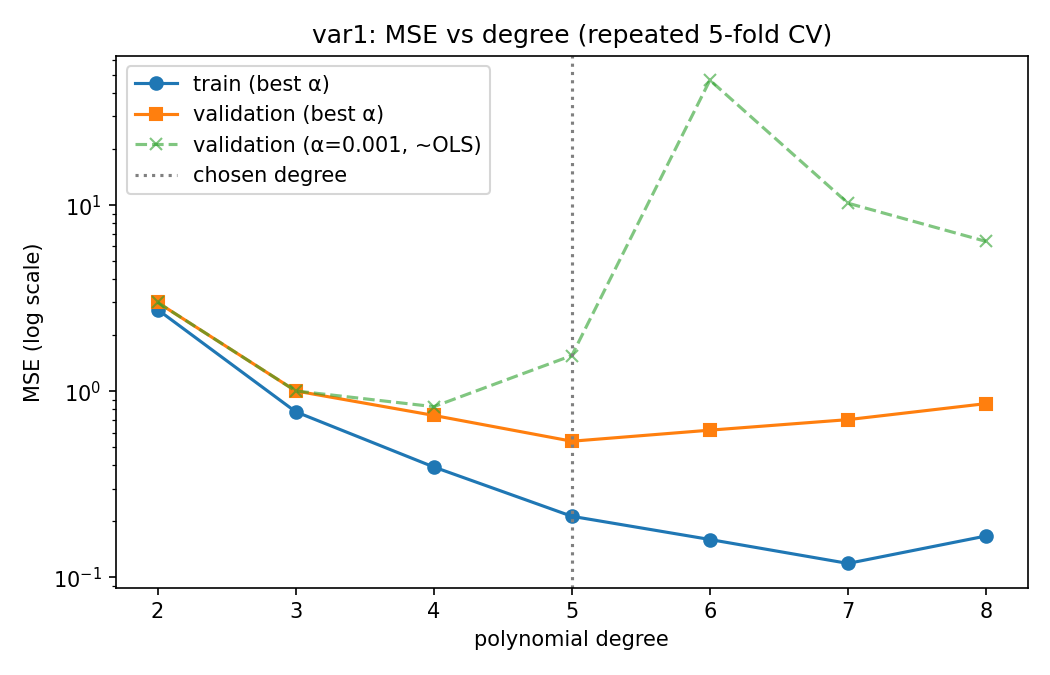
\includegraphics[width=\linewidth]{curve_var1.png}
  \caption{Train/validation MSE vs.\ degree.}
\end{subfigure}\hfill
\begin{subfigure}{0.49\textwidth}
  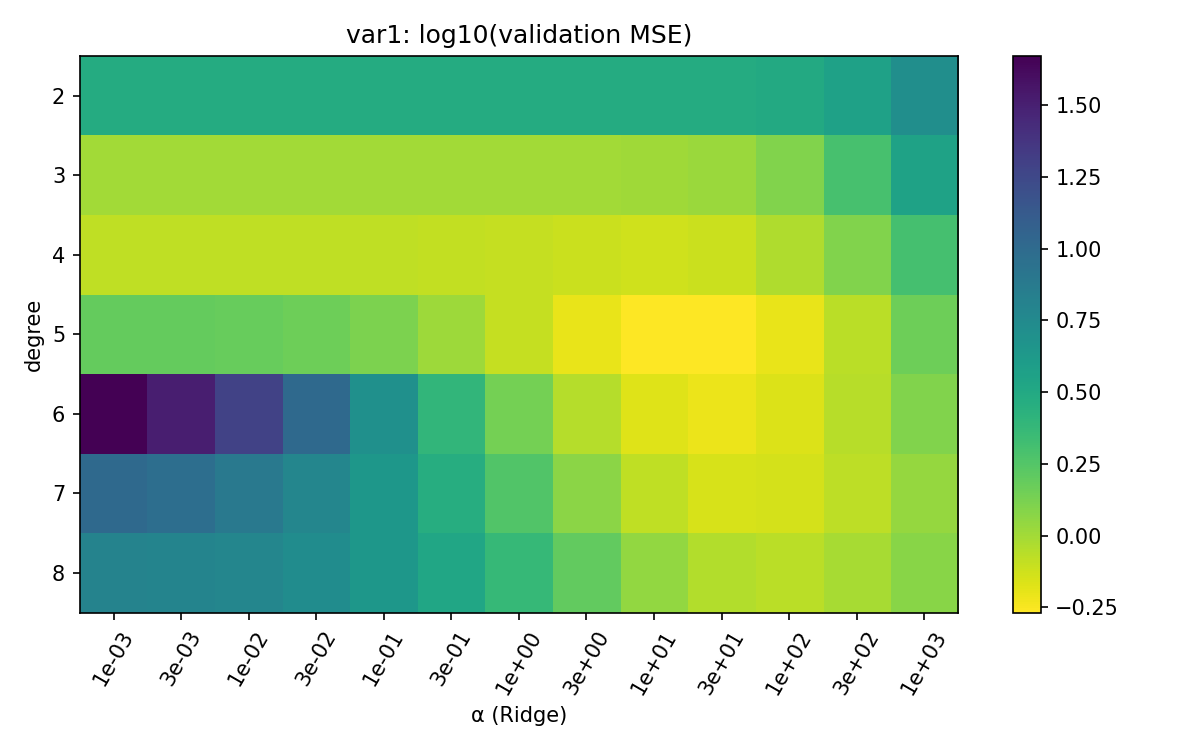
\includegraphics[width=\linewidth]{heatmap_var1.png}
  \caption{$\log_{10}$ validation MSE over $(d,\alpha)$.}
\end{subfigure}
\caption{var1 model selection. The ``$\sim$OLS'' curve (smallest $\alpha$) blows
up beyond $d{=}5$, while the regularised curve has a clear minimum at $d{=}5$.}
\label{fig:v1}
\end{figure}

\subsection{Robustness to the covariate shift}
Because the var1 test set contains more clipped values, a model that is best on
average over the training distribution is not guaranteed to be best on the test
distribution. To check this, we estimated importance weights
\[
w(x) = \frac{p_{\text{test}}(k(x))}{p_{\text{train}}(k(x))},
\qquad k(x) = \#\{j : |x_j| = 1\},
\]
which up-weight training rows with many clipped features (weights range from 0.14
for $k{=}0$ to about 4 for $k\ge4$; effective sample size $\approx 516/1000$). We
then re-ran model selection using an \emph{importance-weighted validation MSE},
which estimates the test error, both with and without weighted fitting.

\begin{itemize}
  \item The best configuration under the weighted criterion is \textbf{the same}:
        $d{=}5$, $\alpha{=}31.62$, fitted without weights
        (importance-weighted validation MSE $0.628$, vs.\ $0.675$ with weighted
        fitting and $0.826$ for the best $d{=}6$ model).
  \item Test predictions change only moderately between neighbouring candidates
        (RMS difference $0.50$ between $d{=}5$ and $d{=}6$), and the strong Ridge
        penalty keeps the predicted range on the test set realistic.
\end{itemize}

\noindent\textbf{Decision (var1):} degree~5, $\alpha = 31.62$, all six features
(461 terms). CV MSE $=0.540\pm0.067$, CV $R^2=0.947$.

% =====================================================================
\section{Problem 2 (var2): Thermal Reservoir}

\subsection{Unregularised baseline}
The var2 target is much smoother in high degree, as the brief suggests. OLS keeps
improving up to $d{=}8$ (validation MSE 0.276, $R^2 = 0.994$). Beyond that, validation
error grows while training error keeps falling. It reaches 17.2 at $d{=}13$, and at
$d{=}15$ the fit is numerically unstable.

\begin{table}[H]
\centering
\small
\begin{tabular}{ccccc}
\toprule
Degree & \# terms & Train MSE & Val MSE & Val $R^2$ \\
\midrule
3  & 19  & 11.546 & 12.453 & 0.739 \\
4  & 34  & 3.338  & 3.756  & 0.920 \\
6  & 83  & 0.442  & 0.578  & 0.988 \\
8  & 164 & 0.164  & \textbf{0.276} & \textbf{0.994} \\
10 & 285 & 0.132  & 0.478  & 0.990 \\
12 & 454 & 0.086  & 2.497  & 0.947 \\
13 & 559 & 0.060  & 17.182 & 0.624 \\
\bottomrule
\end{tabular}
\caption{var2, OLS ($\alpha{=}0$), 5-fold CV (selected degrees).}
\label{tab:v2ols}
\end{table}

\subsection{Ridge-regularised search}
With Ridge the validation curve becomes a broad plateau between $d{=}8$ and
$d{=}13$ instead of a sharp minimum (Table~\ref{tab:v2ridge}, Figure~\ref{fig:v2}).
The global minimum is at $d{=}10$, $\alpha{=}1$.

\begin{table}[H]
\centering
\small
\begin{tabular}{cccccc}
\toprule
Degree & Best $\alpha$ & Train MSE & Val MSE ($\pm$ std) & Val $R^2$ \\
\midrule
6  & 0.032 & 0.441 & $0.596 \pm 0.059$ & 0.9873 \\
7  & 0.10  & 0.230 & $0.339 \pm 0.042$ & 0.9928 \\
8  & 0.10  & 0.170 & $0.263 \pm 0.022$ & 0.9944 \\
9  & 0.32  & 0.165 & $0.259 \pm 0.030$ & 0.9945 \\
\textbf{10} & \textbf{1.00} & 0.164 & $\mathbf{0.247 \pm 0.024}$ & \textbf{0.9947} \\
11 & 1.00  & 0.159 & $0.252 \pm 0.031$ & 0.9946 \\
12 & 3.16  & 0.167 & $0.250 \pm 0.029$ & 0.9946 \\
14 & 3.16  & 0.162 & $0.262 \pm 0.037$ & 0.9944 \\
16 & 3.16  & 0.157 & $0.280 \pm 0.051$ & 0.9940 \\
18 & 10.0  & 0.177 & $0.297 \pm 0.054$ & 0.9936 \\
\bottomrule
\end{tabular}
\caption{var2, best $\alpha$ per degree, repeated 5-fold CV ($3\times$).}
\label{tab:v2ridge}
\end{table}

\begin{figure}[H]
\centering
\begin{subfigure}{0.49\textwidth}
  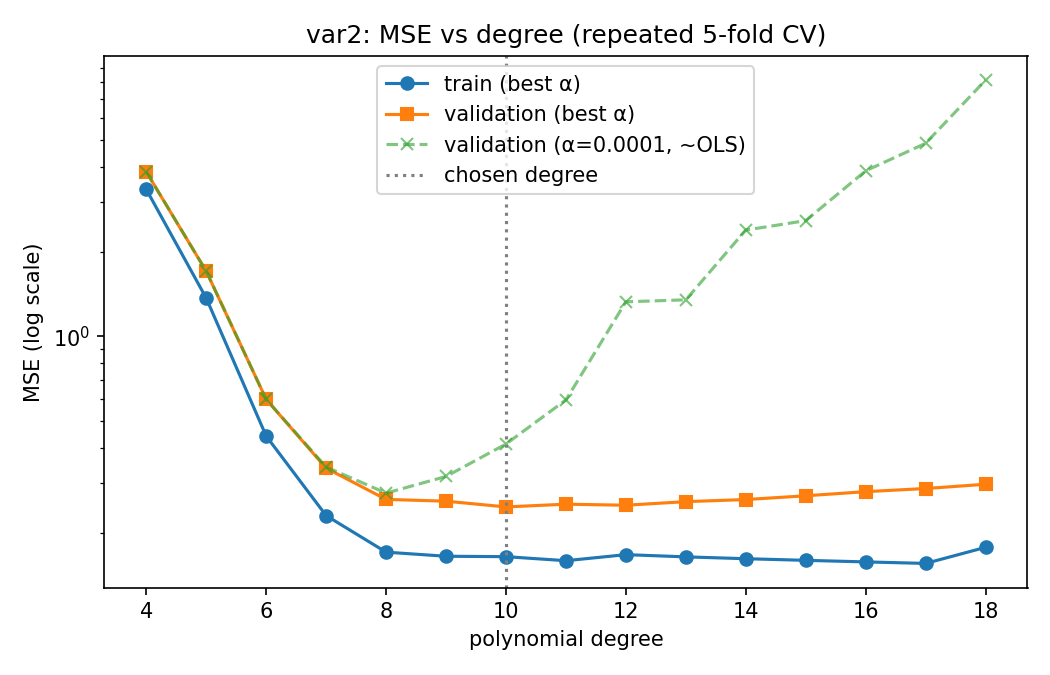
\includegraphics[width=\linewidth]{curve_var2.png}
  \caption{Train/validation MSE vs.\ degree.}
\end{subfigure}\hfill
\begin{subfigure}{0.49\textwidth}
  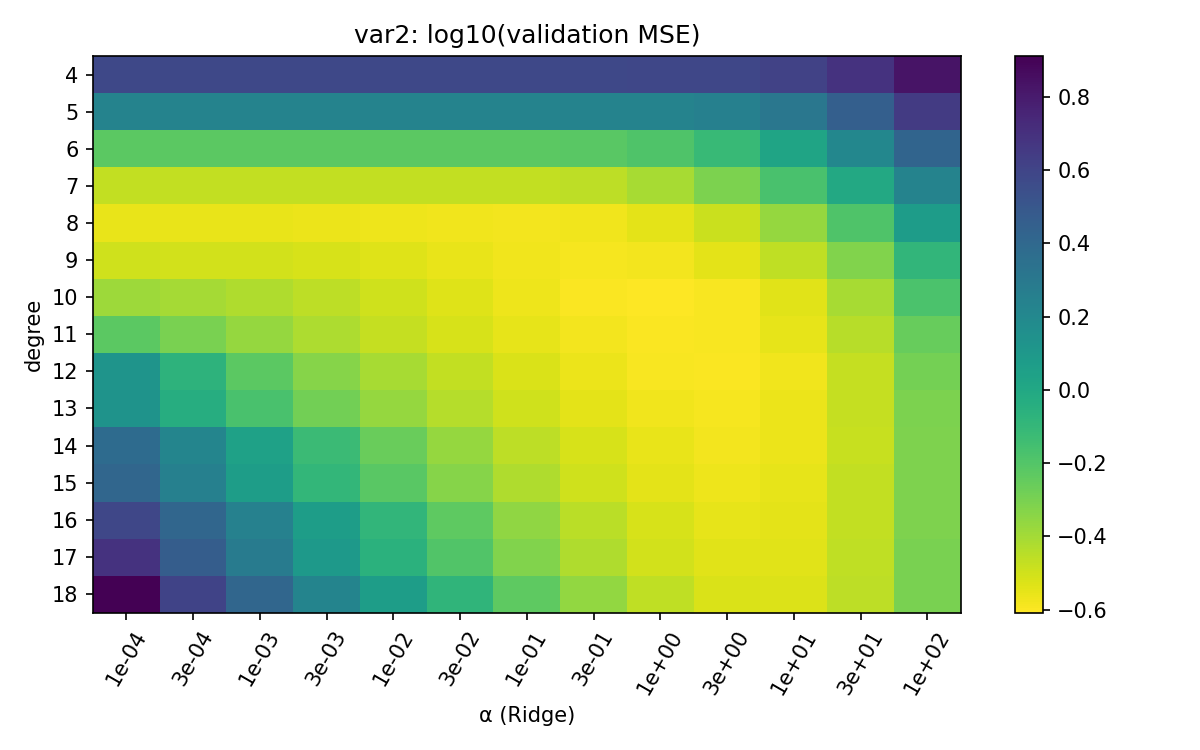
\includegraphics[width=\linewidth]{heatmap_var2.png}
  \caption{$\log_{10}$ validation MSE over $(d,\alpha)$.}
\end{subfigure}
\caption{var2 model selection. Ridge turns the sharp OLS minimum into a wide,
stable plateau ($d\approx 8$--$13$).}
\label{fig:v2}
\end{figure}

\subsection{Stability check}
Because several degrees perform almost equally well, we compared their test
predictions. The RMS difference between the $d{=}8$ and $d{=}10$ models is $0.084$,
and between $d{=}10$ and $d{=}12$ it is $0.071$. Both are far below the
target's standard deviation of 6.9, so the choice within the plateau barely affects
the submitted predictions. There is no train/test shift in var2 (Table~\ref{tab:data}),
so no reweighting is needed.

\noindent\textbf{Decision (var2):} degree~10, $\alpha=1$, all three features
(285 terms). CV MSE $=0.247\pm0.024$, CV $R^2 = 0.995$.

% =====================================================================
\section{Feature Relevance (Ablation)}
To confirm that every input contributes, we removed one feature at a time and
re-ran 5-fold CV at each problem's selected degree:

\begin{table}[H]
\centering
\small
\begin{tabular}{lcccccc|ccc}
\toprule
 & \multicolumn{6}{c|}{var1 ($d{=}5$; all features: 0.776)} & \multicolumn{3}{c}{var2 ($d{=}10$; all: 0.252)} \\
Feature dropped & $x_1$ & $x_2$ & $x_3$ & $x_4$ & $x_5$ & $x_6$ & $x_1$ & $x_2$ & $x_3$ \\
\midrule
Val MSE & 4.23 & 3.33 & 6.08 & 2.14 & 5.45 & 6.24 & 27.40 & 36.07 & 16.23 \\
\bottomrule
\end{tabular}
\caption{Validation MSE after dropping each feature ($\alpha{=}1$ for both problems).}
\label{tab:ablation}
\end{table}

Dropping any single feature makes the error at least $2.7\times$ worse for var1 and
more than $60\times$ worse for var2, so all features are kept in both final models.

% =====================================================================
\section{Final Models and Submission}

\begin{table}[H]
\centering
\small
\begin{tabular}{lccccccc}
\toprule
Problem & Features & Degree & $\alpha$ & \# terms & CV MSE & CV $R^2$ & Full-train $R^2$ \\
\midrule
var1 & $x_1$--$x_6$ & 5  & 31.62 & 461 & $0.540 \pm 0.067$ & 0.947 & 0.979 \\
var2 & $x_1$--$x_3$ & 10 & 1.00  & 285 & $0.247 \pm 0.024$ & 0.995 & 0.997 \\
\bottomrule
\end{tabular}
\caption{Selected models.}
\label{tab:final}
\end{table}

Both models are refit on the full training set and used to produce
\texttt{BT2024199\_pred\_var1.csv} and \texttt{BT2024199\_pred\_var2.csv}
(1000 rows each, single column \texttt{y}, matching the sample submission).

\paragraph{Summary of techniques.}
Polynomial feature expansion with all interaction terms; standardisation of the
expanded features; Ridge regularisation to control variance at high degree; joint
$(d,\alpha)$ grid search using repeated $k$-fold CV; importance-weighted validation
to check robustness to the var1 covariate shift; prediction-stability and
feature-ablation checks.

% =====================================================================
\section{Code and Reproducibility}
All code is available at \repo.
\begin{itemize}
  \item \texttt{train.py} -- final pipeline: grid-search CV, plots, CV tables and prediction files.
  \item \texttt{explore.py} -- dataset statistics and the OLS degree sweep (Tables~\ref{tab:v1ols},~\ref{tab:v2ols}).
  \item \texttt{refine.py} -- Ridge degree sweep and feature ablation (Table~\ref{tab:ablation}).
  \item \texttt{diagnose\_shift.py} -- train/test clipping comparison and prediction stability.
  \item \texttt{shift\_var1.py} -- importance-weighted model selection for var1.
\end{itemize}
To reproduce: \texttt{pip install -r requirements.txt}, then \texttt{python train.py}
(seed 42 fixes all CV splits).

\end{document}
